% !TEX TS-program = xelatex
\documentclass[11pt]{article}
\usepackage{xcolor}
\definecolor{RedViolet}{rgb}{0.78, 0.08, 0.52}
\usepackage{lindrew}
\usepackage{tikz}
\usepackage{pgfplots}
\usepackage{fontspec}
\pgfplotsset{compat=1.18}
\title{Math 4580: Abstract Algebra I}
\author{Lecturer: \textbf{Professor Michael Lipnowski}\\Notes by: Farhan Sadeek}
\date{Spring 2025}

\begin{document}

\maketitle
%%%%%%%%%%%%%%%%%%%%%%%%%%%%

\section{January 6, 2025}
We didn't have any, but Dr.\ Lipnowski did post a module on
\href{https://carmen.osu.edu}{\texttt{carmen}} about the syllabus and the
course. This semester we will be covering the first few chapters of the book
\textit{Abstract Algebra: Theory and Applications} by Thomas Judson. \\

\begin{definition}
    \vocab{Set}: A collection of distinct objects, considered as an object in its own right.\\
    \vocab{Axioms}: A collection of objects \( \mathrm{S} \) with assumed structural rules is defined by axioms.\\
    \vocab{Statement}: In logic or mathematics, an assertion that is either true or false.\\
    \vocab{Hypothesis and Conclusion}: In the statement ``If P, then Q'', P is the hypothesis and Q is the conclusion.\\
    \vocab{Mathematical Proof}: A logical argument that verifies the truth of a statement.\\
    \vocab{Proposition}: A statement that can be proven true.\\
    \vocab{Theorem}: A proposition of significant importance.\\
    \vocab{Lemma}: A supporting proposition used to prove a theorem or another proposition.\\
    \vocab{Corollary}: A proposition that follows directly from a theorem or proposition with minimal additional proof.
\end{definition}

\section{January 8, 2025}
Professor Lipnowski discussed Sam Lloyd's 15 puzzle. Each lecture will include
a mystery digit, contributing up to 5\% bonus to the final grade based on
correct guesses.

Certain course expectations:
\begin{itemize}
    \item All assignments (one every two weeks) and exams (one midterm and one final
          exam) will be take-home.
    \item All the problems from the course textbook.
    \item Collaboration is encouraged, but the work should be your own.
    \item For the exams, we are not supposed to talk to other friends.
\end{itemize}

\subsection{Review of Set Theory}
In this course, we will study \vocab{functions} and \vocab{equivalence
    relations}.\\

\begin{definition}
    A \vocab{function} from a set \( A \) to a set \( B \) is a relation that assigns to each element \( x \) in \( A \) exactly one element \( y \) in \( B \). We write \( f: A \to B \) to denote a function \( f \) from \( A \) to \( B \). Here, \( A \) is the \vocab{domain} and \( B \) is the \vocab{codomain}.\\
    \vocab{Domain}: The set of all possible input values for the function.\\
    \vocab{Codomain}: The set of all possible output values for the function.
\end{definition}

\begin{example}
    Consider the function \( f: \mathbb{Z} \to \mathbb{Z} \) defined by \( f(x) = x^2 \). Here, the domain is the set of all integers \( \mathbb{Z} \), and the codomain is also the set of all integers \( \mathbb{Z} \). For example, \( f(2) = 4 \) and \( f(-3) = 9 \).
\end{example}

\begin{example}
    Another example is the function \( g: \mathbb{R} \to \mathbb{R} \) defined by \( g(x) = \sqrt{x} \). Here, the domain is the set of all non-negative real numbers \( \mathbb{R}_{\geq 0} \), and the codomain is the set of all real numbers \( \mathbb{R} \). For example, \( g(4) = 2 \) and \( g(9) = 3 \).
\end{example}

\begin{fact}
    A function must have a unique output for each input in its domain. This means that for every \( x \in A \), there is exactly one \( y \in B \) such that \( f(x) = y \).
\end{fact}

\begin{center}
    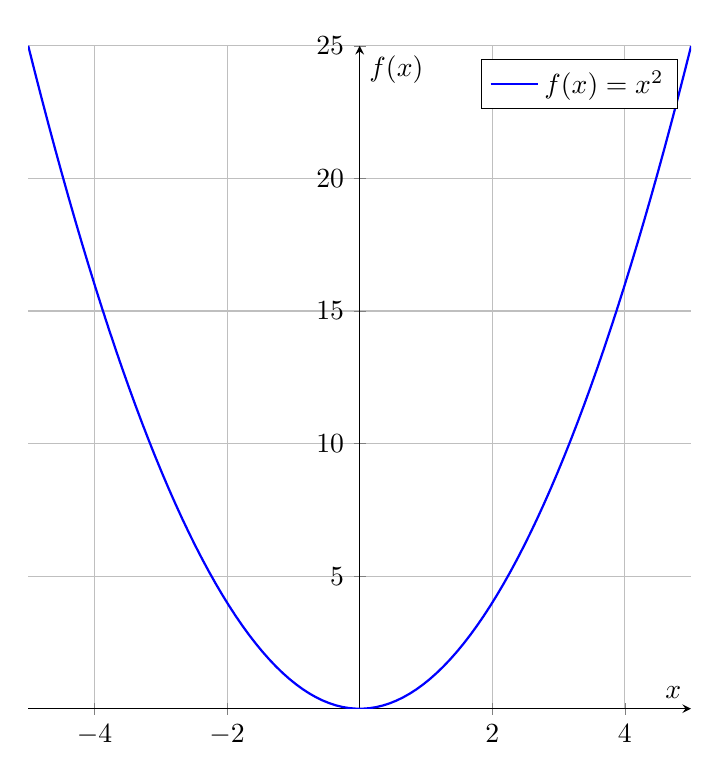
\begin{tikzpicture}
        \begin{axis}[
                axis lines = middle,
                xlabel = $x$,
                ylabel = {$f(x)$},
                domain=-5:5,
                samples=100,
                width=10cm,
                height=10cm,
                grid=both,
                minor grid style={gray!25},
                major grid style={gray!50},
            ]
            \addplot[color=blue, thick] {x^2};
            \addlegendentry{$f(x) = x^2$}
        \end{axis}
    \end{tikzpicture}
\end{center}

\begin{fact}
    A function \( f \) can be represented as a special kind of subset of the Cartesian product \( A \times B \). Specifically, the \vocab{graph} of \( f \) is the set of ordered pairs \( \{(a, b) \mid a \in A, b = f(a)\} \).
\end{fact}

\begin{center}
    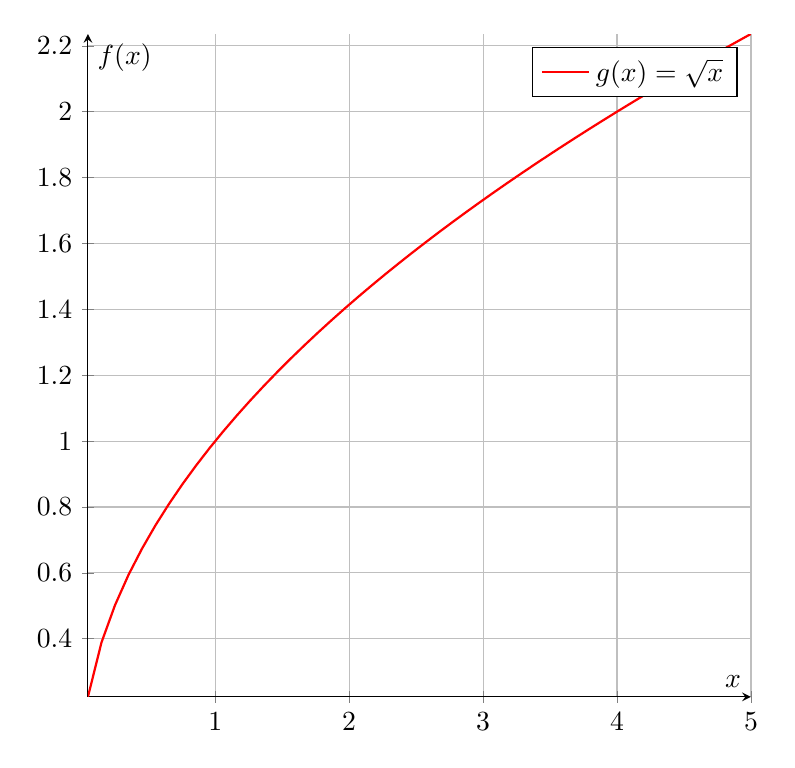
\begin{tikzpicture}
        \begin{axis}[
                axis lines = middle,
                xlabel = $x$,
                ylabel = {$f(x)$},
                domain=-5:5,
                samples=100,
                width=10cm,
                height=10cm,
                grid=both,
                minor grid style={gray!25},
                major grid style={gray!50},
            ]
            \addplot[color=red, thick] {sqrt(x)};
            \addlegendentry{$g(x) = \sqrt{x}$}
        \end{axis}
    \end{tikzpicture}
\end{center}

\begin{proposition}
    A set \( G \subseteq A \times B \) is the graph of a function \( f: A \to B \) if and only if \( G \) intersects every vertical line \( x = a \) at exactly one point.
\end{proposition}

\begin{example}
    Consider the function \( h: \mathbb{R} \to \mathbb{R} \) defined by \( h(x) = e^x \). The graph of this function is the set of ordered pairs \( \{(x, e^x) \mid x \in \mathbb{R}\} \).
\end{example}

\begin{center}
    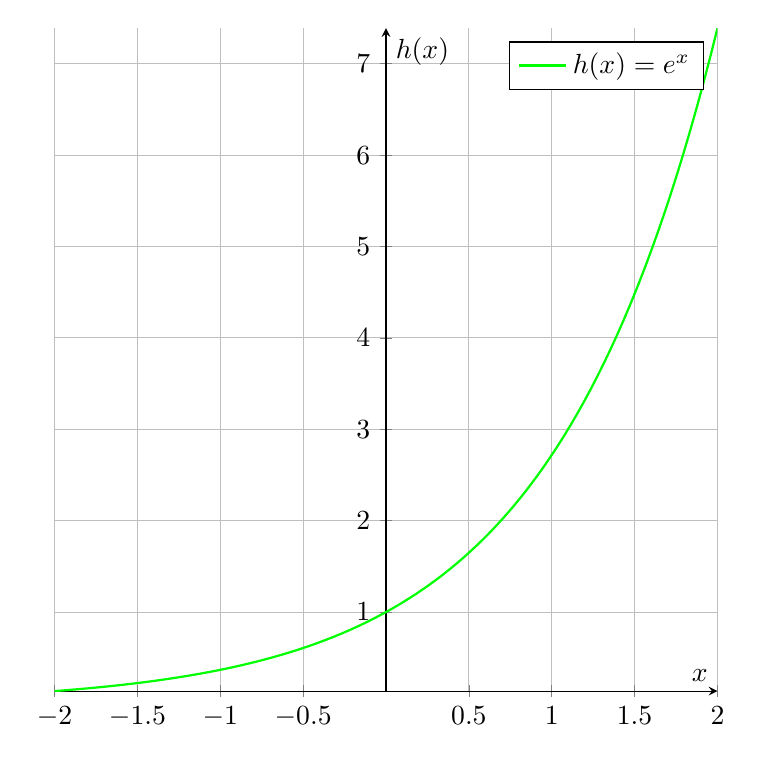
\begin{tikzpicture}
        \begin{axis}[
                axis lines = middle,
                xlabel = $x$,
                ylabel = {$h(x)$},
                domain=-2:2,
                samples=100,
                width=10cm,
                height=10cm,
                grid=both,
                minor grid style={gray!25},
                major grid style={gray!50},
            ]
            \addplot[color=green, thick] {exp(x)};
            \addlegendentry{$h(x) = e^x$}
        \end{axis}
    \end{tikzpicture}
\end{center}

\begin{center}
    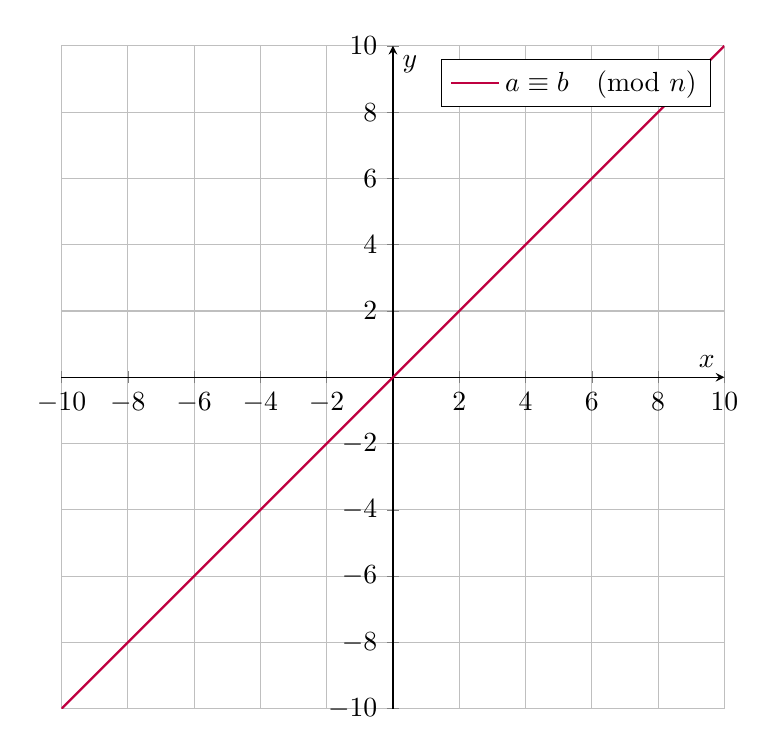
\begin{tikzpicture}
        \begin{axis}[
                axis lines = middle,
                xlabel = $x$,
                ylabel = {$y$},
                domain=-10:10,
                samples=100,
                width=10cm,
                height=10cm,
                grid=both,
                minor grid style={gray!25},
                major grid style={gray!50},
            ]
            \addplot[color=purple, thick] {x};
            \addlegendentry{$a \equiv b \pmod{n}$}
        \end{axis}
    \end{tikzpicture}
\end{center}

\begin{definition}
    The \vocab{vertical line test} is a visual way to determine if a curve in the coordinate plane represents a function. A curve represents a function if and only if no vertical line intersects the curve more than once. This is because a function can only have one output for each input.
\end{definition}

\begin{example}
    Consider the relation defined by the equation \( x^2 + y^2 = 1 \), which represents a circle with radius 1 centered at the origin. This relation does not pass the vertical line test because there are vertical lines that intersect the circle at two points. For example, the vertical line \( x = 0 \) intersects the circle at the points \( (0, 1) \) and \( (0, -1) \). Therefore, the circle is not the graph of a function.
\end{example}
\vspace{10pt}
\begin{center}
    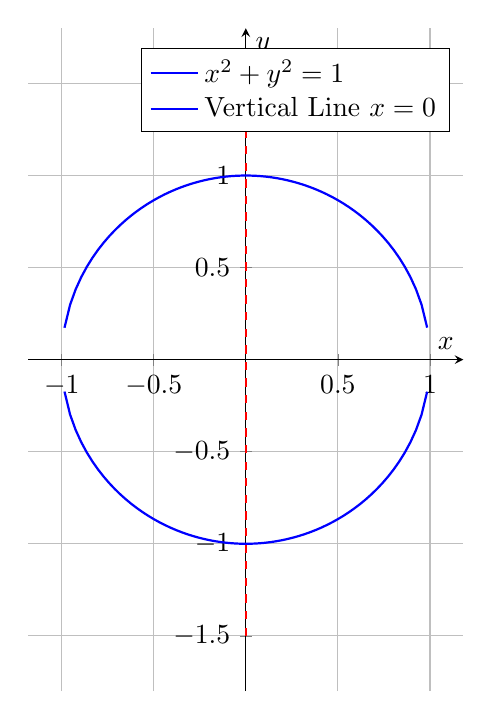
\begin{tikzpicture}
        \begin{axis}[
                axis lines = middle,
                xlabel = $x$,
                ylabel = {$y$},
                domain=-1.5:1.5,
                samples=100,
                width=10cm,
                height=10cm,
                grid=both,
                minor grid style={gray!25},
                major grid style={gray!50},
                legend pos=north east,
                legend cell align={left},
                enlargelimits=true,
                axis equal image
            ]
            \addplot[color=blue, thick] {sqrt(1 - x^2)};
            \addplot[color=blue, thick] {-sqrt(1 - x^2)};
            \addlegendentry{$x^2 + y^2 = 1$}
            \addplot[dashed, color=red, thick] coordinates {(0, -1.5) (0, 1.5)};
            \addlegendentry{Vertical Line $x = 0$}
        \end{axis}
    \end{tikzpicture}
\end{center}
In this case the circle is not the graph of a function because it fails the vertical line test.\\


%\section{January 15, 2025}
%\section{January 17, 2025}
%\section{January 20, 2025}
%\section{January 22, 2025}
%\section{January 24, 2025}
%\section{January 27, 2025}
%\section{January 29, 2025}
%\section{January 31, 2025}
%\section{February 3, 2025}
%\section{February 5, 2025}
%\section{February 7, 2025}
%\section{February 10, 2025}
%\section{February 12, 2025}
%\section{February 14, 2025}
%\section{February 17, 2025}
%\section{February 19, 2025}
%\section{February 21, 2025}
%\section{February 24, 2025}
%\section{February 26, 2025}
%\section{February 28, 2025}
%\section{March 3, 2025}
%\section{March 5, 2025}
%\section{March 7, 2025}
%\section{March 17, 2025}
%\section{March 19, 2025}
%\section{March 21, 2025}
%\section{March 24, 2025}
%\section{March 26, 2025}
%\section{March 28, 2025}
%\section{March 31, 2025}
%\section{April 2, 2025}
%\section{April 4, 2025}
%\section{April 7, 2025}
%\section{April 9, 2025}
%\section{April 11, 2025}
%\section{April 14, 2025}
%\section{April 16, 2025}
%\section{April 18, 2025}
%\section{April 21, 2025}
%\section{April 23, 2025}
%\section{April 25, 2025}
%\section{April 28, 2025}

\end{document}
